In this chapter we discuss similar projects that have been done and how they relate to the project development and execution in relation to our project.We also look at their shortcomings and how they are addressed in our project.


\section{Intelligent Transportation Systems}
Intelligent Transportation Systems are technologies that work with applications and are built with the intention of improving safety in the transport sector, and raising productivity for people

\begin{figure}
    \begin{center}
        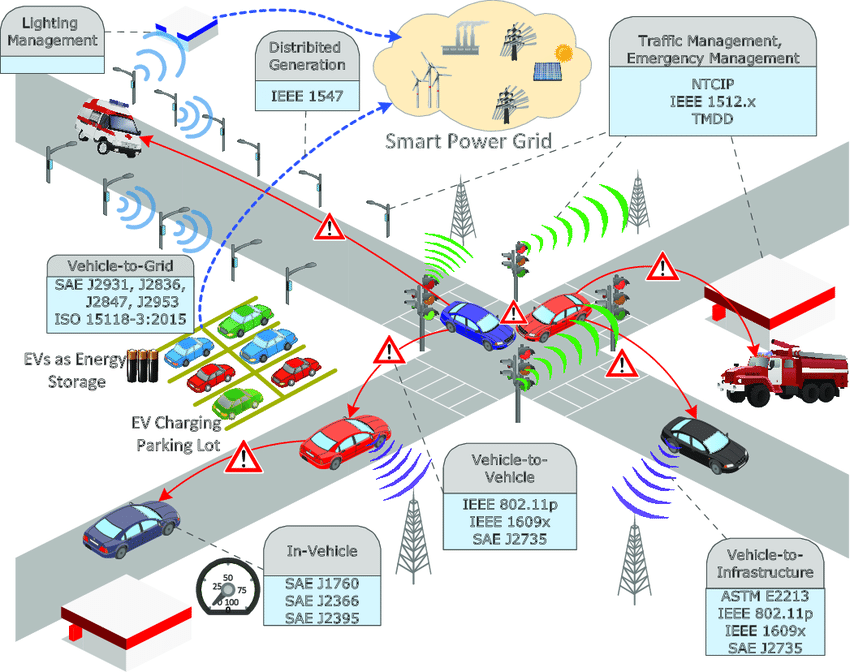
\includegraphics[scale = 0.3]{images/its}
        \caption{A sketch of an intelligent transportation system}
    \end{center}
\end{figure}
Initially proposed in the United States in the twentieth century, a great deal of research is currently going on in this domain as these systems not only improve traffic conditions but are also likely to improve safety, and sustainability in the transportation sector by limiting the inconveniences caused by traffic congestion\cite{i_meneguette_intelligent_2018}.

These systems leverage information and communication technologies, such as embedded sensors, IOT devices\cite{shaheen_intelligent_2004}. They’re used in efforts like real-time data collection from sensors placed in vehicles or infrastructure,and are able to aggregate this data that can then be used to gain insights in information concerning a given city or region. This information can then be used for services and applications aimed at improving the management, plus impproving traffic flow in cities by reducing traffic congestion, which helps lower consumption of fuel and carbon emissions\cite{i_meneguette_intelligent_2018}.

\subsection{Uganda National Roads Authority Express Highway and Makerere University Kampala}

\begin{figure}
    \begin{center}
        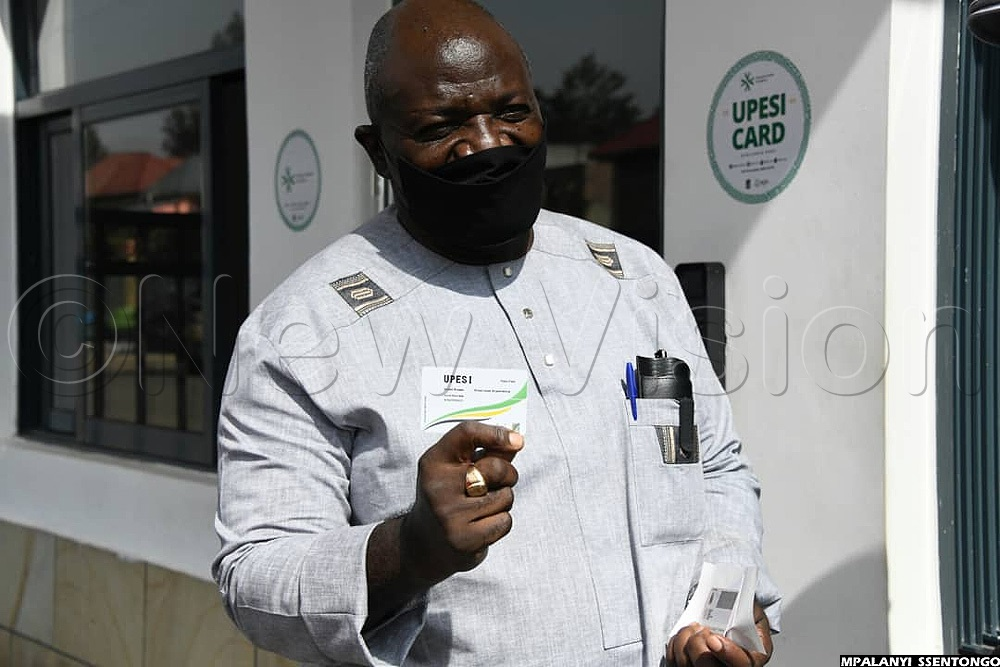
\includegraphics[scale = 0.3]{images/katus}
        \caption{Gen. Katumba Wamala showing an UPESI payment card on the launch of the Entebbe Express Highway}
    \end{center}
\end{figure}
Attempts to put in place a project of this nature in the Ugandan setting have been made though limited by the resources and technology available in the region by the Uganda National Roads Authority through the construction of the Entebbe Express Highway. This implementation is however limited as cashless payments on this road are made electronically through an UPESI RFID card that’s scanned as one tries to access the road\cite{unra_news_2022}.
At Makerere University, individuals who are exempted from paying the parking fee are also given a RFID tag that they place inside their vehicles.This is then scanned by a long-range RFID camera and they’re instantly granted access thereafter\cite{wamai_mak_2014}.

\subsubsection{Project Gap}
The systems mentioned above are not as feasible because:
\begin{itemize}
    \item Cash payments are the commonest way to pay , and these take up time in terms of trying to find change
    \item The alternative payment is an UPESI card, and the process of getting out of the vehicle to scan it is time consuming.
    \item The implementation at Makerere University only accounts for vehicles with RFID tags and the rest have pay with tickets.
\end{itemize}

\subsection{Use of GPS Software and Cell Towers}
Research on how this can be leveraged in easing toll fee payment has been done by others. In 2020, Danang Dismantoro, Istas Pratomo and Surya Sumpeno also proposed a mobile application that allowed payment of these fees via GPS software\cite{el-rabbany_introduction_2002,dismantoro_minimizing_2020}. The system was tested through simulations in Vissim software \cite{ptv_vissim_traffic_2022}, which they believe was able to simulate the real world condition at tollgates. Cell phone towers and GPS technology are used to identify the motorist’ s location and if the motorist happens to be within the toll’s gate vicinity, the money is automatically deducted from their personal account.

\subsubsection{Research Gaps}
\begin{itemize}
    \item No physical implementation of this system was realised
    \item The researchers acknowledge the need for a deeper feasibility study and the fact as it has some shortcomings.
    \item Some scenarios are unaccounted for such as if one is near a cell tower but does not necessarily intend to access the tollgate,they’ll have their money deducted even without actually using the gate.
\end{itemize}


\section{Ubiquitous Computing}
The domain of ubiquitous computing also known as pervasive computing according to Michael Friedewalda and Oliver Raabe is concerned with countless small, wirelessly intercommunicating microprocessors, embedded into objects. Such techniques are applied in similar concepts, such as ``the Internet of things''.The main motive in these domains is assisting people and optimizing economic and social processes through the use of microprocessors and sensors

\begin{figure}
    \begin{center}
        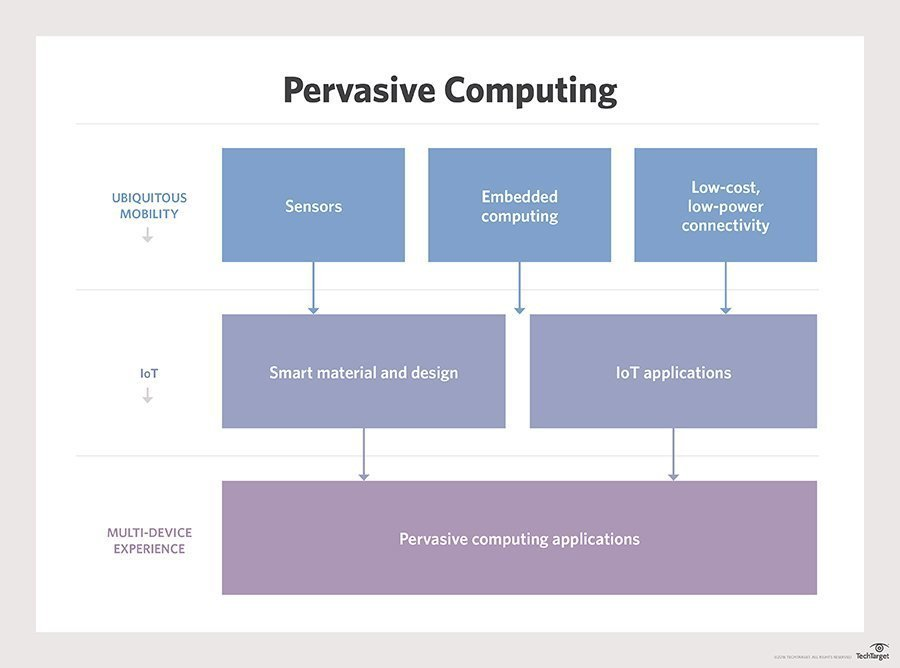
\includegraphics[scale = 0.3]{images/ubq}
        \caption{A sketch of a ubiquitous computing application}
    \end{center}
\end{figure}
These microprocessors are equipped with sensors enabling them to capture information about their current environment or process information and communicate over a network with other similar devices\cite{friedewald_ubiquitous_2011}.

Ubiquitous computing systems consist of features such as:\cite{friedewald_ubiquitous_2011}
\begin{itemize}
    \item The system is decentralised
    \item Computers are embedded in other devices
    \item Real-time information is readily available for users
    \item The system is able to adapt basing on current information.
\end{itemize}

This concept has a number of real world applications in domains such as retail, industrial production, health care and this is achieved through implementations such as tracking applications, wearable devices like smartwatches.

\subsection{Use of RFID sensors}
In the context of toll payment, ubiquitous computing has been put in use in a number of developed countries, and this has been mostly done through the use of RFID technology.

An RFID system has two main components:
\begin{itemize}
    \item A transponder: This is the tag that holds information, found on the object to be identified
    \item A reader/interrogator: This device is able to capture data from the tag.It has a radio frequency module,  control unit and coupling element for linking to the transponder. Additionally, an interface is added to pass on data captured from the transponder to a different system
\end{itemize}


Sabbir Ahmed et al in 2019 also proposed a similar solution.Their proposed system would simplify toll payment through use of RFID tags placed on digitised license plates of all vehicles.Once the tag is scanned, and the motorist has a sufficient balance on their account, the vehicle is granted access\cite{ahmed_automated_2019}.


Another study by Etqad Khan et al. in 2018 proposed a system similar to ours that would ease payment of toll fees using RFID tag that would be linked to motorists' personal accounts where would have a mobile e-wallet on which a given amount would be saved.The system also provides a mobile application to view their past payments\cite{khan_automated_2018}.

\begin{figure}
    \begin{center}
        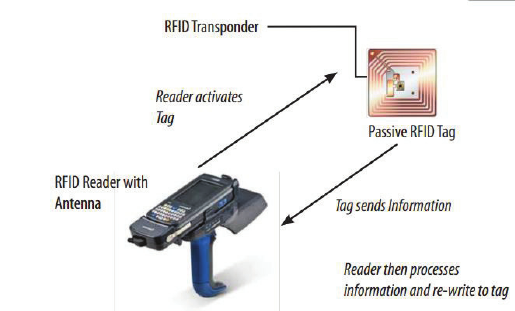
\includegraphics[scale = 0.3]{images/rfid-pic}
        \caption{Components of an RFID system}
    \end{center}
\end{figure}

\subsection{Research Gap}
These two identified studies are constrained in our project scope’s context, because:
\begin{itemize}
    \item It would first off require digitisation of all vehicle license plate, an endeavour that has not yet been taken on by the government of Uganda.
    \item Long range RFID tags and scanners are costly to purchase which would be needed in this use case are costly ,and would thus the need for a low-cost solution that’s accessible to majority of the motorists.
\end{itemize}

\clearpage


\section{Mobile Commerce}
The term E-commerce is used to refer to the buying and selling of goods over the internet. A subset of this is mobile commerce, which is strictly concerned with the same task, but conducted over mobile devices, \cite{varshney_mobile_2000} especially applications on smartphones. This can be attributed to the increased ubiquity of smartphones as well as other handheld devices such as tablets, allowing phone users to do shopping, make bank related transactions. This study is mostly concerned with the process of mobile payments.

Mobile payments refer to using a mobile device, such as a smartphone or tablet, to make financial transactions.This can include making purchases at a store, transferring money to another person, or paying bills.

 \begin{figure}
    \begin{center}
        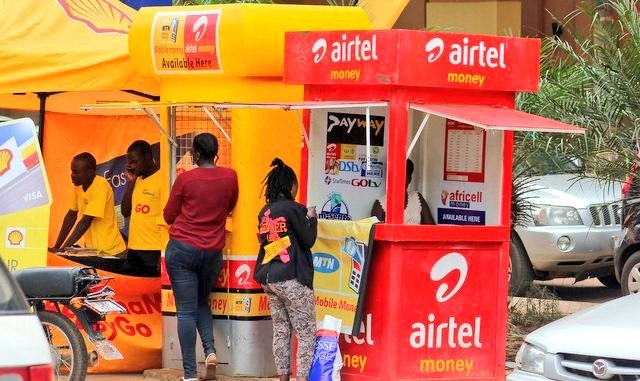
\includegraphics[scale = 0.5]{images/mobile-money}
        \caption{A mobile money kiosk in Kampala. These are a common sight in the city with agents to handle mobile money transactions as bank tellers would in normal banks}
    \end{center}
\end{figure}
In Uganda, the commonest implementation of this is through the mobile money systems\cite{centellegher_mobile_2018}.
In Sub-Saharan Africa, the use of mobile money platforms is promoting financial inclusion, with 548 million registered mobile money accounts in the region. These platforms have seen a 23\% growth in transaction value, reaching 490 billion dollars.

In countries like Uganda, mobile money accounts are held by 43\% of the population, compared to just 11\% who have bank accounts.This demonstrates the significant impact that mobile money platforms are having on financial inclusion in the region\cite{baah_state_2021}.

One of the main advantages of mobile payments is convenience. With mobile payments, there is no need to carry around a physical wallets. Transactions can be completed quickly and easily with just a few taps on your mobile device. This is especially useful in situations where carrying cash is inconvenient or unsafe, such as when traveling or when making a purchase online.

Another advantage of mobile payments is speed. Since mobile payments do not require the physical exchange of cash or the processing of a credit card, transactions can be completed quickly and efficiently. This can save time and effort for both the consumer and the merchant. In addition, mobile payments can enable real-time tracking of transactions, allowing both parties to have immediate access to information about the transaction, such as the amount, the date and time, and the location.

Enhanced security compared to cash payments.Mobile payment systems often use advanced security measures, such as encryption and authentication, to protect against fraud and unauthorized access. This can give consumers peace of mind when making financial transactions, knowing that their personal and financial information is protected.


Payments for these mobile transactions can be completed in a number of ways such as credit cards, debit cards and mobile money platforms such as MTN mobile money, Flutterwave. Our project will rely on the mobile money systems which are ubiquitous in Uganda\cite{baah_state_2021}. It would therefore be advantageous to leverage these platforms

\subsection{Uganda National Roads Authority}
With regards to toll-fee payment, in Uganda, the Entebbe express highway is currently the only existing toll road.Mobile money platforms are leveraged here, but only for loading money onto the UPESI card,\cite{unra_news_2022} that is then used by motorists to pay their fee. This process is quite long, as motorists have to first purchase the card, and repititively load money onto it.A more simplified approach would be to automatically pay directly from the mobile phone

\subsubsection{Project Gaps}
One major shortcoming on the use of mobile commerce with regards to this project, is the payments are only used to add money to the card, which is then later scanned and not directly for access to the road.

\subsection{Use of NFC technology}
Near field communication, or NFC, is a technology that allows two devices to communicate wirelessly when they are close together. This technology is based on radio frequency signals, and it operates over a very short range, typically within a few centimeters of the devices. To use NFC technology, a device must be equipped with an NFC chip, which contains the necessary hardware and software to transmit and receive NFC signals\cite{coskun_survey_2015}. When two NFC-enabled devices are placed near each other, they can exchange information and perform various actions, such as making a payment or transferring data. NFC technology is commonly used in mobile phones, payment cards, and other devices, and it offers a convenient and secure way to conduct transactions and share information.

Rugnesh Rameshram Kanojia and Professor Sujata Pathak in 2018 also proposed a mobile application that would be used for payment of these fees that leverages NFC technology\cite{kanojia_secured_2018}.
An NFC device such as an NFC tag is tapped at the tollgate's NFC tag reader, thereafter user data is verified and the toll charge is deducted

\subsubsection{Research Gap}
NFC payments are very useful as they offer convenience, speed, and security for consumers, and they are becoming increasingly popular as a way to make purchases. Many major banks and retailers now support NFC mobile payments, and the technology is expected to continue to grow in popularity in the coming years, however, as of this writing, they are not yet supported by many of the local payment merchants in Uganda.

\clearpage


\section{Smart Cities}
According to Jonathan Reichental smart cities are a form of Urbanization that leverages technology from a variety of domains such as Internet of Things, cloud computing, mobile applications to improve infrastructure and service delivery, while lowering costs of resource consumption \cite{geng_strategic_2016}. This can include using sensors, data analytics, and other technologies to manage traffic and transportation, reduce pollution, improve public services, and create more efficient and sustainable urban environments.In developing countries like Uganda, implementing smart city technologies can have many benefits, including improving the quality of life for residents.

One of the key ways that smart city technologies can be implemented in Uganda is through the use of sensors and data analytics. For example, sensors can be placed throughout the city to collect data on traffic flow, air quality, and other factors. This data can then be analyzed to identify patterns and trends, and to develop solutions to improve urban services and infrastructure. For example, data on traffic flow could be used to develop more efficient and sustainable transportation systems, such as intelligent traffic management systems or public transportation networks\cite{stimmel_building_2015}.

Implementing smart city technologies in Uganda has the potential to bring many benefits, including improving the quality of life for residents, and promoting economic growth. By using sensors, data analytics, and digital platforms and services, cities like Kampala can become more sustainable, and a better place to live and work.

Digital toll payment systems can play a key role in a smart city, by improving the efficiency and convenience of toll payment, and providing valuable data and insights for urban planners and policymakers. By using technology and data to improve urban services and infrastructure, a smart city can create a better quality of life for its residents and attract investment and economic growth.

\subsection{South Korea}
In South Korea, motorists are able to clear toll fees using a Hi-Pass card. The Hi-Pass system allows drivers to pay tolls without cash and no interaction with the tollbooth is necessary. They are required to have both an OBU (on-board unit) installed on their vehicle's windscreen, and a Hi-Pass card. The OBU is produced by various manufacturers and can be purchased at stores that sell automotive electronics. The Hi-Pass card can be pre-loaded with cash for the toll payment. These cards can often be found at the same stores that sell the OBU\cite{chang_evaluations_2002}.

\subsection{Canada 407 toll Express Highway}
The Canada 407 Express toll route is another demonstration of an futuristic highway that can be used in smart cities. Users create an account on the official website, and purchase a personal transponder, that's attached to the windshield of the vehicles. Cameras on the highway then scan the transponder to identify the vehicle, and make the necessary financial deductions\cite{feldstein_torontos_2015}.

\subsubsection{Project Gaps}
The systems mentioned above and all similar projects help eliminate the tollgate delays and allow the regions they've been implemented evolve into advanced smart cities, however for the scope of our research which is Uganda, taking into account the limited resources such as capital, such projects would be costly to implement thus the need for low-cost solutions


\section{Our Contribution}
Alot of work has been done by other researchers to address the issue of tollgate queues. Many of these solutions leverage RFID technology as an alternative to the physical cash payments. This would however require purchasing costly scanners and tags, thus the need for a similar but cheaper solution.
The biggest benefits to our proposed system:
\begin{itemize}
    \item Use of the local preferred payment platforms such as MTN mobile money, increasing the system's accessibility to individuals in Uganda.
    \item Use of embedded QR code readers as an alternative to RFID tags and scanners which are costly. The QR codes that motorists will use to access the gates will be generated on their mobile phones, thus no need for tickets or such that would be wasteful
    \item Prepaid payments that would eliminate the delays and queues: Our proposed system would eliminate the queues that commonly arise as motorists make their payments.
\end{itemize}

\begin{figure}
    \begin{center}
        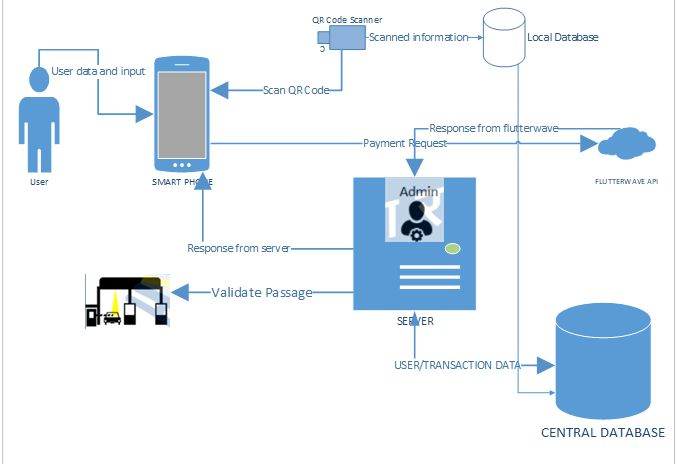
\includegraphics[scale = 0.6]{images/etolssys}
        \caption{System Architecture Diagram for the proposed solution }
    \end{center}
\end{figure}